\chapter{Zobrazovací systém}

Zobrazovací systém slouží výpisům aktuálních událostí hráče. Mezi tyto události patří čas, osobní statistiky hráče či jméno hráče kterého naposledy trefil, nebo kým byl trefen.

\begin{figure}[H]
    \begin{center}
        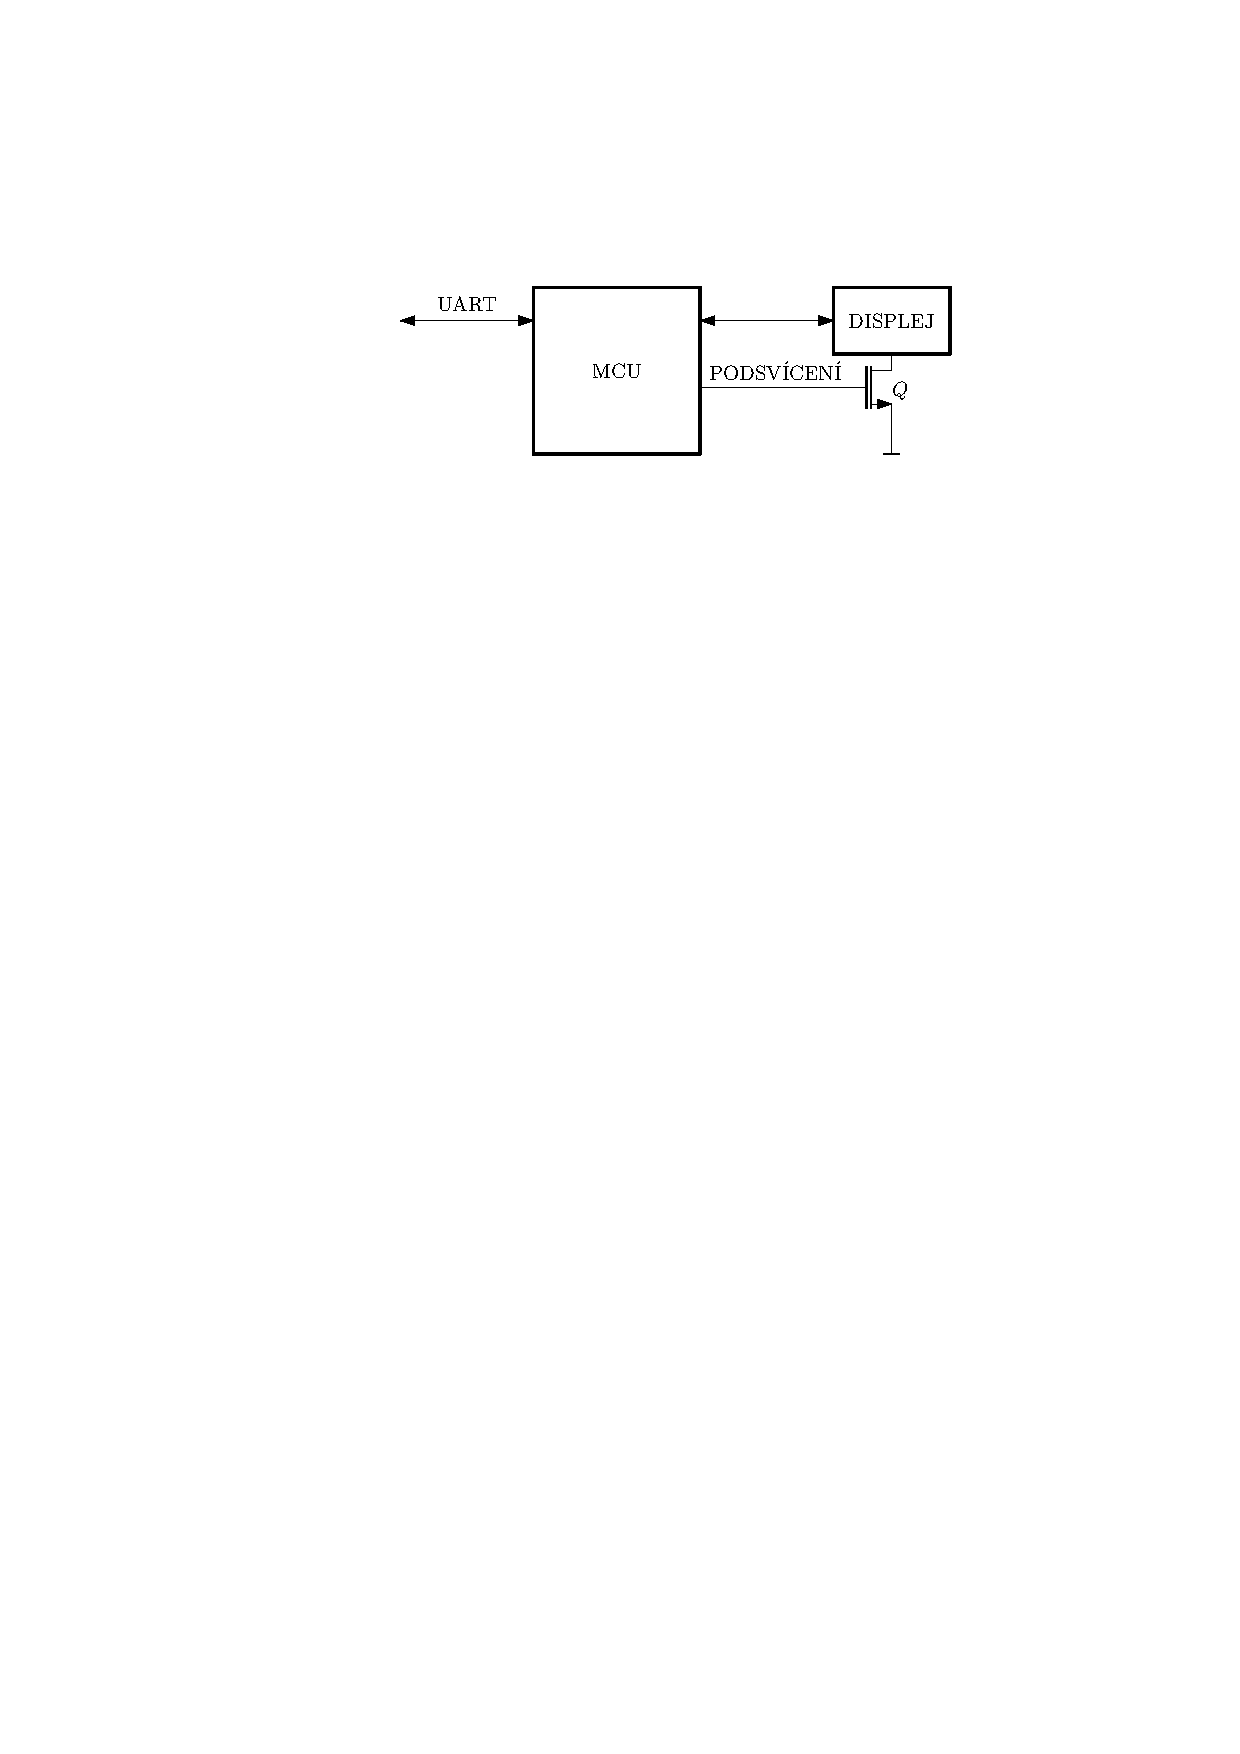
\includegraphics[width=\textwidth]{img/display}
    \end{center}
    \caption{Blokové schéma zobrazovacího systému}
\end{figure}

Zobrazovač je postaven na MCU STM32F042F6P a displeji RC1602. Zobrazovací systém je navržen tak, že s řídícím MCU vesty komunikuje pomocí UART. Je to samostatný modul, díky tomu není problém vyrobit vesty bez zobrazovače, či místo tohoto modulu navrhnout modul jiný. Další výhodou této koncepce je možnost zobrazovaná data rychle uložit do RAM MCU zobrazovače a poté je zapisovat. Jelikož komunikace ze znakovým LCD založeným na řadiči HD44780 je značně pomalá, tak nebude zdržován hlavní MCU vesty. Naopak nevýhodou tohoto řešení je cena jednoho MCU navíc.

Zobrazovač má možnost díky řídícímu tranzistoru ovládat podsvícení zobrazovače a tím snižovat spotřebu zařízení.
